\chapter{Lista de Exercícios 1}


\begin{enumerate}[label=\emph{\arabic*})]

	\item Considere o material denominado "Exemplo de Relatório Estatístico – Estatística Descritiva"

	      Para os estudantes da disciplina Probabilidade e Estatística (MA70H), turma S09, o censo apurado para a variável "quantidade de disciplinas matriculadas no semestre letivo 2/2020" foi: 8, 5, 5, 7, 9, 7, 8, 9, 6, 8, 6, 6, 7, 7, 4, 3.

	      A turma S09 tem 20 estudantes matriculados em MA70H, mas o levantamento de dados foi feito em apenas 16 estudantes, pois um estudante chegou atrasado à aula de 24/02, quando foi realizado o levantamento de dados, e outros três estudantes não compareceram à aula de 24/02.

	      \begin{enumerate}[label=\emph{\alph*})]

		      \item Classifique a variável;

		            \textbf{Resolução:}	A variável é quantitativa discreta

		      \item Identifique a unidade de medida da variável;

		            \textbf{Resolução:}	número de disciplinas matriculadas

		      \item Identifique a escala de medição da variável;

		            \textbf{Resolução:}	A variável possui escala de proporcionalidade

		      \item \label{item_graficos} Para o censo acima, construa as tabelas 1, 2, 3 e 4 e os gráficos 1, 2, 3, 4 e 5, presentes no material acima referido. Não se esqueça de colocar título completo e fonte em cada tabela e em cada gráfico; caso necessário, colocar notas e chamadas no rodapé das tabelas e gráficos;

		            \textbf{Resolução:}

		            \begin{table}[]
			            \centering
			            \caption{Estudantes da disciplina Probabilidade e Estatística (MA70H), turma S09, semestre  letivo  2/2020, da  Universidade  Tecnológica  Federal  do  Paraná, campus Curitiba, segundo a quantidade de disciplinas matriculadas}
			            \resizebox{0.7\textwidth}{!}{%
				            \begin{tabular}{cc}
					            \hline
					            \multicolumn{1}{c|}{Estudante} & Nº de disciplinas matriculadas                \\
					            \hline
					            1                              & 8                                             \\
					            2                              & 5                                             \\
					            3                              & 5                                             \\
					            4                              & 7                                             \\
					            5                              & 9                                             \\
					            6                              & 7                                             \\
					            7                              & 8                                             \\
					            8                              & 9                                             \\
					            9                              & 6                                             \\
					            10                             & 8                                             \\
					            11                             & 6                                             \\
					            12                             & 6                                             \\
					            13                             & 7                                             \\
					            14                             & 7                                             \\
					            15                             & 4                                             \\
					            16                             & 3                                             \\
					            17                             & Não informado, pois não participou da da aula \\
					            18                             & Não informado, pois chegou atrasado na aula   \\
					            19                             & Não informado, pois chegou atrasado na aula   \\
					            20                             & Não informado, pois chegou atrasado na aula   \\
					            \hline
				            \end{tabular}
			            }
			            \label{tab:d-1}
			            \begin{minipage}{0.7\linewidth}
				            \emph{Fonte: Autoria própria}
			            \end{minipage}
		            \end{table}

		            \begin{table}[]
			            \centering
			            \caption{Estudantes da disciplina Probabilidade e Estatística (MA70H), turma S09, semestre  letivo  2/2020,  da  Universidade  Tecnológica  Federal  do  Paraná, campus Curitiba, segundo a quantidade de disciplinas matriculadas}
			            \resizebox{0.7\textwidth}{!}{%
				            \begin{tabular}{cc}
					            \hline
					            \multicolumn{1}{c|}{Nº de disciplinas matriculadas} & Frequência \\
					            \hline
					            3                                                   & 1          \\
					            4                                                   & 1          \\
					            5                                                   & 2          \\
					            6                                                   & 3          \\
					            7                                                   & 4          \\
					            8                                                   & 3          \\
					            9                                                   & 2          \\
					            \hline
					            Total                                               & 16         \\
					            \hline
				            \end{tabular}
			            }
			            \label{tab:d-2}
			            \begin{minipage}{0.7\linewidth}
				            \emph{Fonte: Autoria própria}
			            \end{minipage}
		            \end{table}

		            \begin{table}[]
			            \centering
			            \caption{Medidas   estatísticas   para   descrever   os   estudantes   da   disciplina Probabilidade   e   Estatística   (MA70H),   turma   S09,   semestre   letivo   2/2020,   da Universidade Tecnológica Federal do Paraná, campus Curitiba, segundo a quantidade de disciplinas matriculadas}
			            \resizebox{0.7\textwidth}{!}{%
				            \begin{tabular}{ccc}
					            \hline
					            \multicolumn{1}{c|}{Medida estatística}                    & \multicolumn{1}{c|}{Valor calculado} & Unidade de medida \\ \hline
					            \multicolumn{1}{c|}{Quantidade de dados ($N$)}             & 16                                   & -                 \\
					            \multicolumn{1}{c|}{Mínimo ($Min$)}                        & 3                                    & disciplina        \\
					            \multicolumn{1}{c|}{Máximo ($Max$)}                        & 9                                    & disciplina        \\
					            \multicolumn{1}{c|}{Amplitude ($A$)}                       & 6                                    & disciplina        \\
					            \multicolumn{1}{c|}{Moda ($Mo$)}                           & 7                                    & disciplina        \\
					            \multicolumn{1}{c|}{Percentil 10 ($P_{10}$)}               & 3                                    & disciplina        \\
					            \multicolumn{1}{c|}{Primeiro Quartil ($Q_{1}$)}            & 3                                    & disciplina        \\
					            \multicolumn{1}{c|}{Mediana ($\tilde{x}$)}                 & 5                                    & disciplina        \\
					            \multicolumn{1}{c|}{Terceiro Quartil ($Q_{3}$)}            & 7                                    & disciplina        \\
					            \multicolumn{1}{c|}{Percentil 90 ($P_{90}$)}               & 9                                    & disciplina        \\
					            \multicolumn{1}{c|}{Média ($\mu$)}                         & 6.5625                               & disciplina        \\
					            \multicolumn{1}{c|}{Variância populacional ($\sigma^{2}$)} & 2.929167                             & disciplina$_{2}$  \\
					            \multicolumn{1}{c|}{Desvio padrão populacional ($\sigma$)} & 1.711481                             & disciplina        \\
					            \multicolumn{1}{c|}{Coeficiente de variação ($CV$)}        & 26.07971                             & \%                \\
					            \multicolumn{1}{c|}{Coeficiente de assimetria ($As$)}      & -0.4393908                           & -                 \\
					            \multicolumn{1}{c|}{Coeficiente de curtose ($K$)}          & -0.5138676                           & -                 \\ \hline
				            \end{tabular}%
			            }
			            \label{tab:d-3}
			            \begin{minipage}{0.7\linewidth}
				            \emph{Fonte: Autoria própria}
			            \end{minipage}
		            \end{table}

		            \begin{table}[]
			            \centering
			            \caption{Escores  padronizados  para  a  quantidade  de  disciplinas  matriculadas referente  aos  estudantes  da  disciplina  Probabilidade  e  Estatística  (MA70H),  turma S09, semestre letivo 2/2020, da Universidade Tecnológica Federal do Paraná, campus Curitiba}
			            \resizebox{0.7\textwidth}{!}{%
				            \begin{tabular}{ccc}
					            \hline
					            \multicolumn{1}{c|}{\begin{tabular}[c]{@{}c@{}}N°  de disciplinas matriculadas\\ $(X)$\end{tabular}} & \multicolumn{1}{c|}{Frequência} & \begin{tabular}[c]{@{}c@{}}Escore padronizado z, com\\ $Z_{i}=\frac{x_{i}-\mu}{\sigma}$\end{tabular} \\ \hline
					            3                                              & 1                               & -2.0815308                \\
					            4                                              & 1                               & -1.4972414                \\
					            5                                              & 2                               & -0.9129521                \\
					            6                                              & 3                               & -0.3286628                \\
					            7                                              & 4                               & 0.2556266                 \\
					            8                                              & 3                               & 0.8399159                 \\
					            9                                              & 2                               & 1.4242053                 \\ \hline
					            Total                                          & 16                              &                           \\ \cline{1-2}
				            \end{tabular}%	  			      
			            }
			            \label{tab:d-4}
			            \begin{minipage}{0.7\linewidth}
				            \emph{Fonte: Autoria própria}
			            \end{minipage}
		            \end{table}

		            \begin{figure}[H]
			            \centering
			            \subfloat[\centering]{{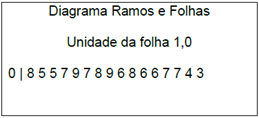
\includegraphics[width=0.4\linewidth]{fig/d-graph-1-1}}}
			            \qquad
			            \subfloat[\centering]{{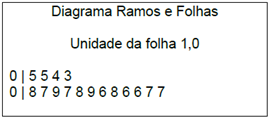
\includegraphics[width=0.4\linewidth]{fig/d-graph-1-2}}}
			            \caption{
				            Estudantes da disciplina Probabilidade e Estatística (MA70H), turma S09, semestre  letivo  2/2020,  da  Universidade  Tecnológica  Federal  do  Paraná, campus Curitiba, segundo a quantidade de disciplinas matriculadas
			            }
			            \label{fig:d-graph-1}
			            \begin{minipage}{0.7\linewidth}
				            \emph{Fonte: Autoria própria}
			            \end{minipage}
		            \end{figure}

		            \begin{figure}[H]
			            \centering
			            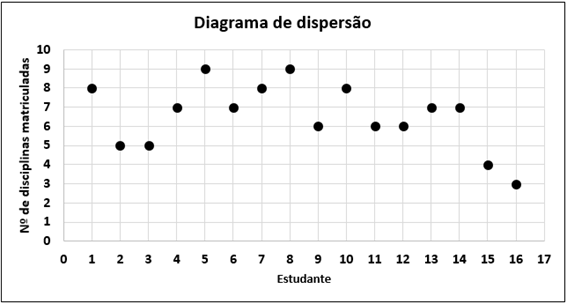
\includegraphics[width=0.7\linewidth]{fig/d-graph-2}
			            \caption{
				            Estudantes da disciplina Probabilidade e Estatística (MA70H), turma S09, semestre  letivo  2/2020,  da  Universidade  Tecnológica  Federal  do  Paraná, campus Curitiba, segundo a quantidade de disciplinas matriculadas
			            }
			            \label{fig:d-graph-2}
			            \begin{minipage}{0.7\linewidth}
				            \emph{Fonte: Autoria própria}
			            \end{minipage}
		            \end{figure}

		            \begin{figure}[H]
			            \centering
			            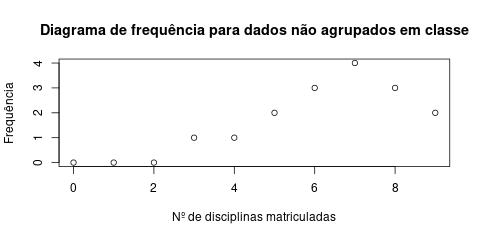
\includegraphics[width=0.7\linewidth]{fig/d-graph-3}
			            \caption{
				            Estudantes da disciplina Probabilidade e Estatística (MA70H), turma S09, semestre  letivo  2/2020,  da  Universidade  Tecnológica  Federal  do  Paraná, campus Curitiba, segundo a quantidade de disciplinas matriculadas
			            }
			            \label{fig:d-graph-3}
			            \begin{minipage}{0.7\linewidth}
				            \emph{Fonte: Autoria própria}
			            \end{minipage}
		            \end{figure}

		            \begin{figure}[H]
			            \centering
			            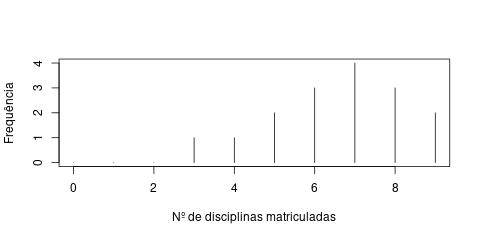
\includegraphics[width=0.7\linewidth]{fig/d-graph-4}
			            \caption{
				            Estudantes da disciplina Probabilidade e Estatística (MA70H), turma S09, semestre  letivo  2/2020,  da  Universidade  Tecnológica  Federal  do  Paraná, campus Curitiba, segundo a quantidade de disciplinas matriculadas
			            }
			            \label{fig:d-graph-4}
			            \begin{minipage}{0.7\linewidth}
				            \emph{Fonte: Autoria própria}
			            \end{minipage}
		            \end{figure}

		            \begin{figure}[H]
			            \centering
			            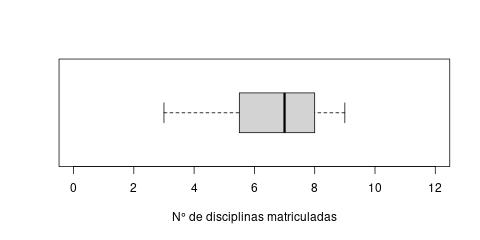
\includegraphics[width=0.7\linewidth]{fig/d-graph-5}
			            \caption{
				            Medidas   estatísticas   para   descrever   os   estudantes   da   disciplina Probabilidade   e   Estatística   (MA70H),   turma   S09,   semestre   letivo   2/2020,   da Universidade Tecnológica Federal do Paraná, campus Curitiba, segundo a quantidade de disciplinas matriculadas
			            }
			            \label{fig:d-graph-5}
			            \begin{minipage}{0.7\linewidth}
				            \emph{Fonte: Autoria própria}
			            \end{minipage}
		            \end{figure}

		      \item Interprete os dados e escreva uma conclusão sobre eles, baseando-se nas tabelas e gráficos construídos no item \ref{item_graficos};


		            \textbf{Resolução:} Com base na análise dos dados estatísticos de quantidade de disciplinas matriculadas no semestre letivo 2/2020 (8, 5, 5, 7, 9, 7, 8, 9, 6, 8, 6, 6, 7, 7, 4, 3), algumas conclusões foram tiradas: 3 foi a menor quantidade de disciplinas e 9 a maior; a moda foi de 7 disciplinas; 6,25\% da turma se matricularam em até 3 disciplinas; 43,75\% se matricularam em até 6 disciplinas; 87,5\% se matricularam em até 8 disciplinas e 100\% da turma se matriculou em até 8,5, consequentemente, 9 disciplinas.


		            Com a média sendo 6,56, a moda e a mediana iguais a 7, podemos concluir que pela proximidade dos valores, em termos de desvio padrão (1,65), os valores estão distribuídos aproximadamente simétricos em torno da média.


		      \item Fazer capa e folha de rosto nas normas de apresentação de trabalhos acadêmicos.

	      \end{enumerate}

\end{enumerate}



